% =======================================================
% 3. INTERFACCIA UTENTE
% =======================================================
\section{Panoramica dell'Interfaccia}
L'interfaccia di Second Brain è progettata per massimizzare la concentrazione (distraction-free) garantendo al contempo un rapido accesso agli strumenti AI.

% \begin{figure}[H]
%    \centering
%    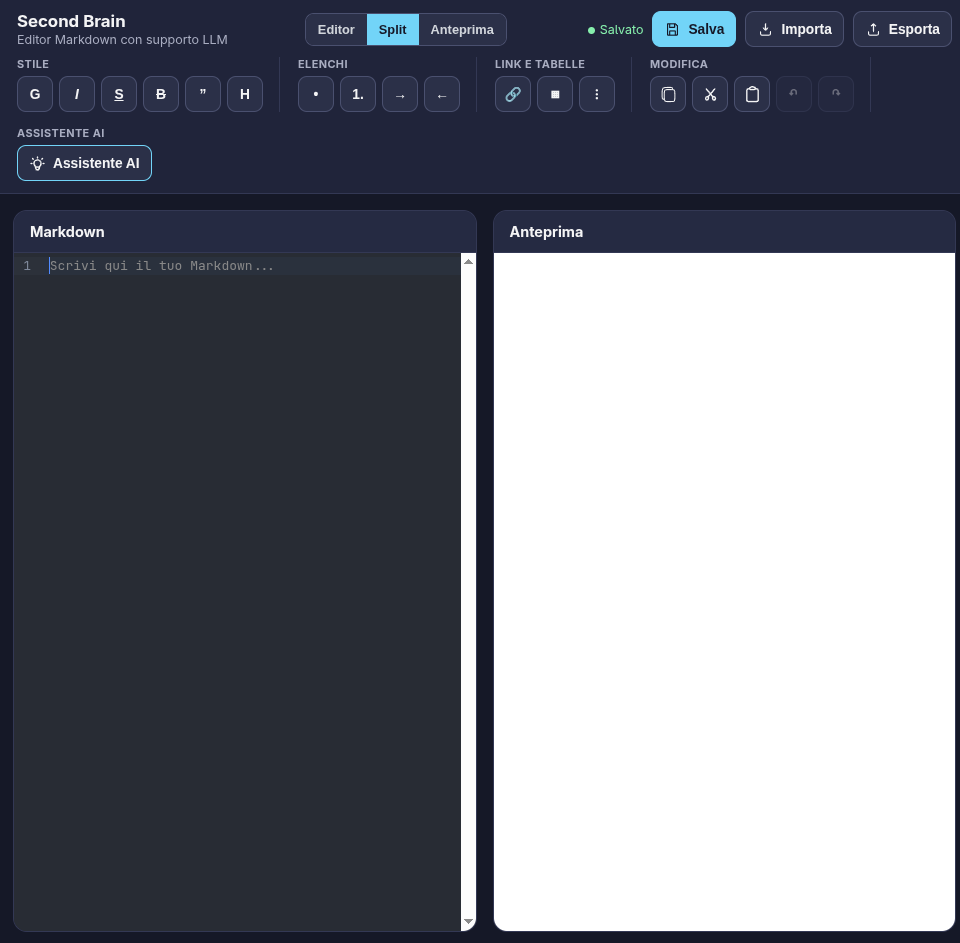
\includegraphics[width=0.9\textwidth]{img/overview_interfaccia.png}
%    \caption{Layout principale dell'applicazione}
% \end{figure}

\subsection{Barra Superiore (Topbar)}
[Descrivere gli elementi presenti in alto: es. Titolo del documento modificabile, indicatore di stato di salvataggio].

\subsection{Barra Laterale (Sidebar)}
[Descrivere il menu laterale: navigazione tra editor e storico, pulsanti di upload/download, toggle per la modalità scura/chiara].

\subsection{Modalità di Visualizzazione}
Il sistema offre diverse modalità per adattarsi al flusso di lavoro dell'utente:
\begin{itemize}
    \item \textbf{Solo Editor:} Massimizza lo spazio dedicato alla scrittura del codice sorgente Markdown.
    \item \textbf{Solo Render:} Nasconde l'editor per mostrare il documento finale impaginato.
    \item \textbf{Split View:} [Spiegare l'anteprima affiancata in tempo reale].
\end{itemize}